% ****** Start of file apssamp.tex ******
%
%   This file is part of the APS files in the REVTeX 4.2 distribution.
%   Version 4.2a of REVTeX, December 2014
%
%   Copyright (c) 2014 The American Physical Society.
%
%   See the REVTeX 4 README file for restrictions and more information.
%
% TeX'ing this file requires that you have AMS-LaTeX 2.0 installed
% as well as the rest of the prerequisites for REVTeX 4.2
%
% See the REVTeX 4 README file
% It also requires running BibTeX. The commands are as follows:
% 
%  1)  latex apssamp.tex
%  2)  bibtex apssamp
%  3)  latex apssamp.tex
%  4)  latex apssamp.tex
%
\documentclass[%
 reprint,
%superscriptaddress,
%groupedaddress,
%unsortedaddress,
%runinaddress,
%frontmatterverbose, 
%preprint,
%preprintnumbers,
%nofootinbib,
%nobibnotes,
%bibnotes,
 amsmath,amssymb,
 aps,
%pra,
%prb,
%rmp,
%prstab,
%prstper,
%floatfix,
]{revtex4-2}
%Tikz
% Tikz Feynman Diagrams
% by Flip Tanedo
% 4 January 2011, work in progress
% Revised Dec 10

%%%%%%%%%%%%%%%%%%%%%%%%%%%%%%%%%%%%%%%%%%%%
%%% TIKZ - for drawing Feynman diagrams %%%%
%%% ... use with pdflatex   			%%%%
%%%%%%%%%%%%%%%%%%%%%%%%%%%%%%%%%%%%%%%%%%%%

\usepackage{tikz}
\usetikzlibrary{arrows,shapes}
\usetikzlibrary{trees}
\usetikzlibrary{snakes}
\usetikzlibrary{matrix,arrows} 				% For commutative diagram
											% http://www.felixl.de/commu.pdf
\usetikzlibrary{positioning}				% For "above of=" commands
\usetikzlibrary{calc,through}				% For coordinates
\usetikzlibrary{decorations.pathreplacing}  % For curly braces
\usepackage[tikz]{bclogo} 					% For cute logo boxes
\usepackage{pgffor}							% For repeating patterns

\usetikzlibrary{decorations.pathmorphing}	% For Feynman Diagrams
\usetikzlibrary{decorations.markings}
\usetikzlibrary{intersections}				% For interesections


% Based on:
% http://www.texample.net/tikz/examples/feynman-diagram/

\tikzset{
	% >=stealth', %% more traditional arrows, I don't like them
    vector/.style={decorate, decoration={snake}, draw},
    fermion/.style={postaction={decorate},
        decoration={markings,mark=at position .55 with {\arrow{>}}}},
    fermionbar/.style={draw, postaction={decorate},
        decoration={markings,mark=at position .55 with {\arrow{<}}}},
    fermionnoarrow/.style={},
    gluon/.style={decorate,
        decoration={coil,amplitude=4pt, segment length=5pt}},
    scalar/.style={dashed, postaction={decorate},
        decoration={markings,mark=at position .55 with {\arrow{>}}}},
    scalarbar/.style={dashed, postaction={decorate},
        decoration={markings,mark=at position .55 with {\arrow{<}}}},
    scalarnoarrow/.style={dashed,draw},
%
%%% 	Special vectors (when you need to fine-tune wiggles)
%	provector/.style={decorate, decoration={snake,amplitude=2.5pt}, draw},
%	antivector/.style={decorate, decoration={snake,amplitude=-2.5pt}, draw},
%	    electron/.style={draw=black, postaction={decorate},
%        decoration={markings,mark=at position .55 with {\arrow[draw=black]{>}}}},
%	bigvector/.style={decorate, decoration={snake,amplitude=4pt}, draw},
	vectorscalar/.style={loosely dotted,draw=black, postaction={decorate}},
}
\usepackage[
  locale=DE,                   % deutsche Einstellungen
  separate-uncertainty=true,   % immer Unsicherheit mit \pm
  per-mode=symbol-or-fraction, % / in inline math, fraction in display math
]{siunitx}

\usepackage{graphicx}% Include Figure files
\usepackage{dcolumn}% Align table columns on decimal point
\usepackage{bm}% bold math
\usepackage{amssymb}
%\usepackage{hyperref}% add hypertext capabilities
%\usepackage[mathlines]{lineno}% Enable numbering of text and display math
%\linenumbers\relax % Commence numbering lines

%\usepackage[showframe,%Uncomment any one of the following lines to test 
%%scale=0.7, marginratio={1:1, 2:3}, ignoreall,% default settings
%%text={7in,10in},centering,
%%margin=1.5in,
%%total={6.5in,8.75in}, top=1.2in, left=0.9in, includefoot,
%%height=10in,a5paper,hmargin={3cm,0.8in},
%]{geometry}

\begin{document}

\preprint{APS/123-QED}

\title{Measurement of lepton universality in\\ $b \to s l^+ l^-$ decays}% Force line breaks with \\
%\thanks{A footnote to the article title}%

\author{Moritz Bosse}
 \altaffiliation[Also at ]{Physics Department, TU Dortmund University.}%Lines break automatically or can be forced with \\
  \email{moritz.bosse@tu-dortmund.de}
\affiliation{%
 TU Dortmund University, Germany\\
}%

%\collaboration{MUSO Collaboration}%\noaffiliation

%\author{Charlie Author}
% \homepage{http://www.Second.institution.edu/~Charlie.Author}
%\affiliation{
% Second institution and/or address\\
% This line break forced% with \\
%}%
%\affiliation{
% Third institution, the second for Charlie Author
%}%
%\author{Delta Author}
%\affiliation{%
% Authors' institution and/or address\\
% This line break forced with \textbackslash\textbackslash
%}%
%
%\collaboration{CLEO Collaboration}%\noaffiliation

\date{\today}% It is always \today, today,
             %  but any date may be explicitly specified

%inserting abstract
\begin{abstract}
    In this proceeding a review of a simultaneous analysis of the 
    $B^+ \to K^+ l^+ l^-$ and $B^0 \to K^{\star 0} l^+ l^-$ decays to test muon-electron universality
    is presented. Using a dataset of B-meson decays collected with the LHCb detector from Run 1 and 2 with
    ${\SI{9}{\femto\barn}}^{-1}$ integrated luminosity, multivariate selections and strict particle identification requirements were applied to enhance signal purity 
    and statistical sensitivity. Backgrounds from misidentified hadronic decays were studied and included in the analysis. 
    The measurements establish results for the specific non-resonant $q^2$ range and are in good agreement to the Standard Model, yielding a notable improvement over 
    previous measurements. %Notably, the results align with the predictions of the Standard Model.
    %\begin{description}
    %\item[Usage]
    %Secondary publications and information retrieval purposes.
    %\item[Structure]
    %You may use the \texttt{description} environment to structure your abstract;
    %use the optional argument of the \verb+\item+ command to give the category of each item. 
    %\end{description}
\end{abstract}
%inserting abstract

%\keywords{Suggested keywords}%Use showkeys class option if keyword
                              %display desired
\maketitle

%\tableofcontents

The Standard Model (SM) is the most successful theory for describing the fundamental particles and their interactions, excluding gravity.
It has been extensively tested through numerous experiments and has provided highly precise predictions that match experimental observations. Phenomena such as Dark Matter, Baryon asymmetry or
massive neutrinos are pointing towards a more fundamental UV-complete theory. %the SM has shortcomings and that we are far from having a full UV-complete theory. 
A very sensitive probe to test New Physics is through high precision measurements, where small deviations from the SM could arise 
through unknown beyond the Standard Model (BSM) particles or mechanisms. 
\\
Within the Standard Model, the gauge Bosons have identical coupling constants to all three families of leptons ($e$, $\mu \and \tau$),
which is known as Lepton Universality (LU). Decays into different dilepton final states should then only differ by their respective masses. 
\newline
Up to now, there is no known reason behind the necessity for LU, however it has been observed experimentally at per mille levels 
in W and Z boson decays .. cite. Since there is no fundamental law (as far as we know) that forces BSM particles to couple equally to all
lepton flavors, one can gain insight and constrain possible BSM theories by the measurement of LU aswell as provide more evidence for the accurary of SM predictions.
\newline
In the recent years there have been a number of LU measurements in $b \to s l^+ l^-$
transitions (cite) that throughout show a pattern of deviations from the SM predictions. 
Most notably the measurement using $B^+ \to K^+ l^+ l^-$ decays, showing $3.1 \sigma$ significance ....
The broad consensus is ... that such deviations can not be explained by theoretical uncertainies, 
so it is off special interest to study LU in these transitions. In this paper, a simultaneous test of muon-electron
universality in non-resonant $B^+ \to K^+ l^+ l^-$ and $B^0 \to K^{\star 0} l^+ l^-$ decays unsing LHCb data is presented.
\newline
The Large Hadron Collider beauty (LHCb) is one of the four big experiments at the Large Hadron Collider (LHC) at CERN. It is a single-arm forward
spectrometer covering a pseudorapidity between $2 < \eta < 5$ and is mainly used to investigate b (beauty) and c (charm) quarks.
The proton-proton collisions take place within the Vertex Locater (VELO) where primary aswell as secondary vertices can be distinguished and precisely reconstructed.
Through the combination of a $\SI{4}{\tesla\meter}$ dipole magnet and multiple tracking stations (TT, T1-T3), the charge and momentum of the particle can be measured.
For the full particle identification, Cherenkov detectors (RICH), different Calorimeters (ECAL, HCAL) and alternating layers of iron and multiwire proportional chambers to measure muons are used.
To reduce the amount of data produced from the pp collisions, a hardware trigger (L0) based on calorimeter and muon system parameters, followed by a software trigger (HLT) that selects events based on a full event reconstruction is implemented.
\newline
To measure LU the observable $R$ is constructed as follows
\begin{equation}
    \label{eqn:1}
    R_{K, K^*}\left(q_a^2, q_b^2\right)=\frac{\int_{q_a^2}^{q_b^2} \frac{\mathrm{d} \Gamma\left(B^{(+, 0)} \rightarrow K^{(+, * 0)} \mu^{+} \mu^{-}\right)}{\mathrm{d} q^2} \mathrm{~d} q^2}{\int_{q_a^2}^{q_b^2} \frac{\mathrm{d} \Gamma\left(B^{(+, 0)} \rightarrow K^{(+, * 0)} e^{+} e^{-}\right)}{\mathrm{d} q^2} \mathrm{~d} q^2}.
\end{equation}
These observables are measured in two $q^2$ regions: $0.1<q^2<1.1 \mathrm{GeV}^2 / c^4$ (low- $q^2$); $1.1<q^2<6.0 \mathrm{GeV}^2 / c^4$ (central- $\left.q^2\right)$. 
The central $q^2$ region excludes light meson resonances in the lower limit and the $J/\Psi$ resonance above $6.0 \mathrm{GeV}^2$. In previous measurements the lower limit of the low $q^2$ region 
included the dimuon mass threshhold of $0.045 \mathrm{GeV}^2 / c^4$, which is now pushed upwards.
This is done to reduce the form-factor and charm loop uncertainties 
that occur near the photon pole .. .
The biggest remaining uncertainies stem from modelling radiative effects .....
\\
Previous deviations in $R_{K, K^*}$ ... showed a coherent pattern, motivating theoretical heavy BSM contributions. Different examples are shown using the typical EFT framework in Figure \ref{fig:1}.
To produce a deviation in $R_{K, K^*}$, new contributions to the Wilson coefficients $\mathcal{C}_9$ (vector-like) and $\mathcal{C}_{10}$ (axial vector-like) are proposed.
\begin{figure}
    \centering
    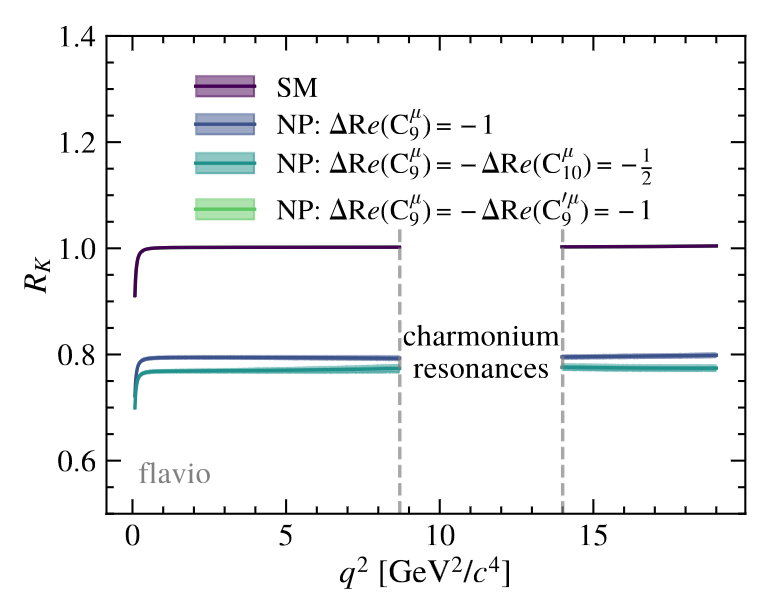
\includegraphics[width=0.5\textwidth]{theory2.png}
    \caption{Theoretical predictions for $R_K$ and $R_{K^*}$ as a function of $q^2$ in different BSM scenarios \cite{lhcbcollaboration2022measurement}.}
    \label{fig:1}
\end{figure}
In this analysis the resonances of $J/\Psi$ ($6<q^2<11 \mathrm{GeV}^2 / c^4$) and $\Psi$($2S$) ($11<q^2<15 \mathrm{GeV}^2 / c^4$) are used for calibration  
and to maximise the cancellation of efficiencies between the processes. 
For this efficiency cancellation the double ratio 
\begin{align*}
    R_{\left(K, K^*\right)} \equiv& \frac{\frac{\mathcal{N}}{\varepsilon}\left(B^{(+, 0)} \rightarrow K^{(+, * 0)} \mu^{+} \mu^{-}\right)}{\frac{\mathcal{N}}{\varepsilon}\left(B^{(+, 0)} \rightarrow K^{(+, * 0)} J / \psi\left(\rightarrow \mu^{+} \mu^{-}\right)\right)} \times \\[1pt]
     &\frac{\frac{\mathcal{N}}{\varepsilon}\left(B^{(+, 0)} \rightarrow K^{(+, * 0)} J / \psi\left(\rightarrow e^{+} e^{-}\right)\right)}{\frac{\mathcal{N}}{\varepsilon}\left(B^{(+, 0)} \rightarrow K^{(+, * 0)} e^{+} e^{-}\right)},%
\end{align*}
is defined. Where the number of events $\mathcal{N}$ is determined from mass fits and the efficiency correction for the affiliated process $\epsilon$ is evaluated from
data-driven corrected simulations. Due to the single ratio of the resonant $J/\Psi$ mode 
\begin{equation*}
    r_{J / \psi}^{K, K^*} \equiv \frac{\frac{\mathcal{N}}{\varepsilon}\left(B^{(+, 0)} \rightarrow K^{(+, * 0)} J / \psi\left(\rightarrow \mu^{+} \mu^{-}\right)\right)}{\frac{\mathcal{N}}{\varepsilon}\left(B^{(+, 0)} \rightarrow K^{(+, * 0)} J / \psi\left(\rightarrow e^{+} e^{-}\right)\right)},
\end{equation*}
which is measured to be unity \cite{cali}%check the cite here below
, one is able to perform cross checks of the calibration. Additionaly the double ratio method can be checked for robustness by looking at double ratios with 
the $\Psi$(2S) resonance as the signal mode.
\newline
The analysis has to withstand multiple challenges.
One of the main difficulties lies in the reconstruction of the muon and the electron tracks.
However, especially the reconstruction of the electron modes poses a great difficulty. The main reason lies in the emitting 
of Bremsstrahlung that lead to a larger width in the mass fits due to a loss of reconstructed momentum. 
In order to address this problem, a specialized algorithm for Bremsstrahlung reconstruction is employed. 
The primary objective of this algorithm is to restore the momentum that has been lost through the emission of Bremsstrahlung.
 This is achieved through the identification of photons within the electromagnetic calorimeter. 
 These photons are likely linked to the emission of Bremsstrahlung radiation from the signal electrons. 
 Despite the utilization of this reconstruction technique, the precision of the mass resolution for electron modes continue to be notably compromised 
 when contrasted with the performance in muon modes. Consequently, it becomes crucial to manage potential background contamination in the electron mode.
\\
Two other crucial aspects are the limited resolution of the electromagnetic calorimeter and the reduced L0 trigger efficiency for electrons. 
To tackle the reduced trigger efficiencies, the analysis utilizes a method that merges candidates triggered by the signal electrons with those prompted by other non-signal particles in the event (TIS). 
This strategy substantially recuperates signal events in cases where the electrons did not satisfy the trigger thresholds in the ECAL.
A multivariate classifier is employed to differentiate between $B^{(+, 0)} \rightarrow K^{(+, * 0)}l^+ l^-$ decay processes and combinatorial background occurrences using 
kinematic and vertex quality information.
The training procedure involves simulated signal events, along with data containing reconstructed B meson invariant masses exceeding $5400 (5600) {\si{\mega\electronvolt}}/c^2$, 
serving as approximations for muon (electron) combinatorial backgrounds. 
To increase the dataset, background events from the low- and central-$q^2$ regions are combined.
Prior to the training phase, preselection and particle identification (PID) criteria are applied, with an equal number of signal and background events.
A second classifier is trained for the electron modes to seperate signal from the partially reconstructed $B \rightarrow (K, K^{*0})l^+ l^{-}X$ decays, 
where $X$ describes an additional hadron. For this kinematic and geometric features of the signal are used. 
\\
Both classifiers are optimized simultaneously with the predicted signal significance for SM decay rates, for each $q^2$ region and data taking period.
To avoid bias, a k-fold cross validation is used.
It is also necesseary to study background that remains even after all the selection criteria have been applied. This is again done through simulation.
Specific vetoes are used to reduce many of these backgrounds. One example for a semileptonic veto in the $B^+$ decay mode is shown in Figure \ref{fig:2}.
\begin{figure}
    \centering
    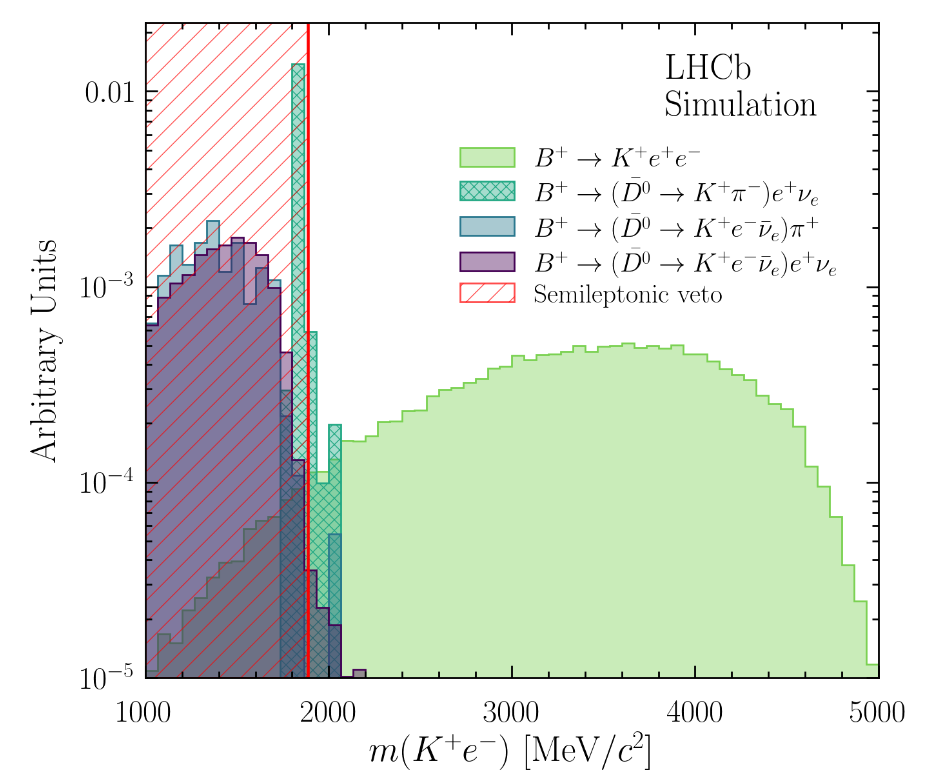
\includegraphics[width=0.5\textwidth]{veto2.png}
    \caption{Semileptonic veto for backgrounds in the $B^+$ decay mode.}
    \label{fig:2}
\end{figure}
% Produces the bibliography via BibTeX.
One important aspect of the analysis is the accurate determination of efficiencies and the calibration of the simulation. For each data-taking year
the simulation is calibrated with real data control samples. No single data control sample can account for all the different aspects of the detector 
performance, so that a multi-step correction is utilized in the following way
\begin{equation*}
\omega_i = \frac{\epsilon_{\text{Data}}}{\epsilon_{\text{Simulation}}}.
\end{equation*}
The different aspects denoted by $i$ are each weighted differently for the $J$/$\Psi$ resonant decay. There are six main components that are corrected for. These 
include the PID ($\omega_{\text{PID}}$), electron track reconstruction ($\omega_{\text{Track}}$), event multiplicity and B meson kinematics ($\omega_{\text{mult}\&\text{kin}}$),
 L0 and HLT trigger performance ($\omega_{\text{L}0}$, $\omega_{\text{HLT}}$), aswell as a final set of calibrations concerning the performance of the reconstruction ($\omega_{\text{reco}}$).
Lastly the $q^2$ resolution and bin-migration ($\omega_{\text{reso}}$) is accounted for.
Muon and Hadron track reconstruction efficiencies have been found to agree well with data and hence are not included. 
All of the different correction effects are illustrated in Figure \ref{fig:2} . It becomes apparent that the double ratios $R_{\left(K, K^*\right)}$ are notably
less influenced by the corrections, than the single ratios  $r_{J / \psi}^{K, K^*}$. The single ratio efficiencies change by 25\%, while
all double ratio efficiencies are adjusted by at most 5\%.
This demonstrates the robustness of the double ratio method over the single ratio when it comes to systematic
uncertainties in the efficiencies. The final observable is hence constructed from the double ratio.
\begin{figure}
    \centering
    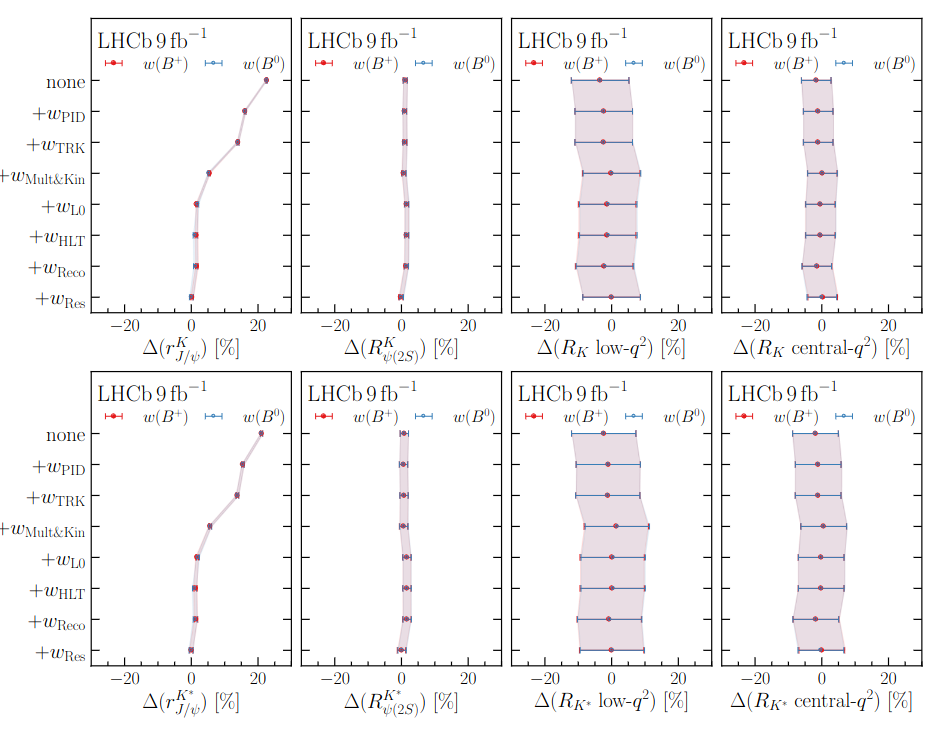
\includegraphics[width=0.5\textwidth]{eff.png}
    \caption{Calibration of efficiencies in the single and double ratios for the resonant decay modes.}
    \label{fig:3}
\end{figure}
After all selection criteria have been applied, the nonresonant muon samples
contain only signal and combinatorial backgrounds. The invariant mass spectrum of
the nonresonant muon signals is modeled using simulated data, while the combinatorial
background is modeled using an exponential fit.
The nonresonant electron samples have a higher complexity owing to migration from the resonant $J$/$\Psi$ decay into the central $q^2$ region, residual
misidentified hadronic decays or partially reconstructed background without misidentification.
The invariant mass spectrum for the electron decays are modelled simillarly. The leakage from the $J$/$\Psi$ decay and the partially reconstructed background
however are modeled using a kernel-density estimator ... 
that is derived from simulation. The misidentified background is studied individually and the effects are found to be very small. The large number 
of misidentification prone decays and their poorly understood dynamics can still have a noticable overall contribution, even when compared to the 
expected statistical sensitivy. They are therefore estimated using data and modeled using an empirical function. 
The invariant mass distribution for the non-resonant electron decays is depicted in Figure \ref{fig:4}.
\begin{figure}
    \centering
    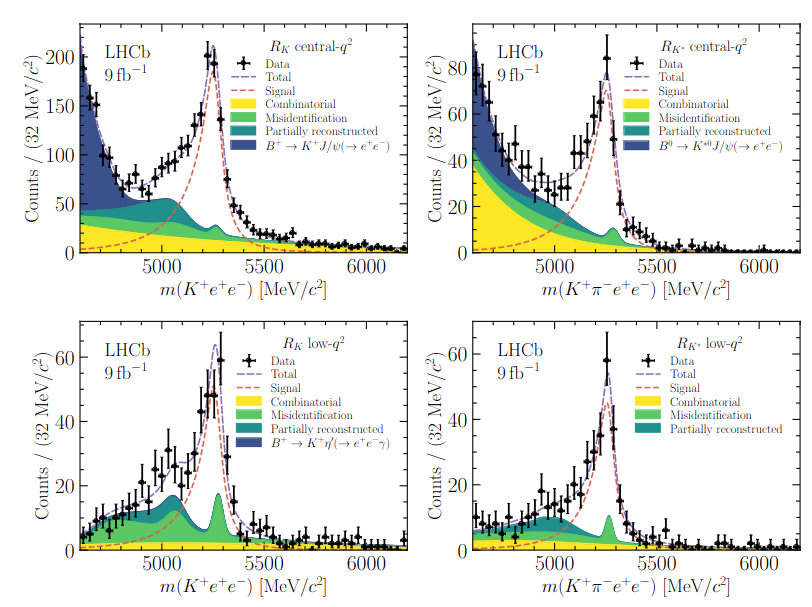
\includegraphics[width=0.5\textwidth]{mass.png}
    \caption{Invariant mass distributions of the non-resonant $B^+ \rightarrow K^+ e^+ e^-$ (left) and $B^0 \rightarrow K^{*0} e^+ e^-$ (right) decays.}
    \label{fig:4}
\end{figure}
The final fit using all the mass fits and efficiencies, yields the LU Observables \eqref{eqn:1} in both $q^2$ regions
\begin{equation}
    \begin{array}{r}
    \text{low-} q^2\left\{\begin{array}{l}
    R_K=0.994_{-0.082}^{+0.090}\text{(stat)}_{-0.027}^{+0.029} \text{(syst),} \\
    R_K^*=0.927_{-0.087}^{+0.093}\text{(stat)}_{-0.035}^{+0.036}\text{(syst),}
    \end{array}\right. \\
    \text {central-} q^2\left\{\begin{array}{l}
    R_K=0.949_{-0.041}^{+0.042}\text{(stat)}_{-0.022}^{+0.022}\text{(syst),} \\
    R_K^*=1.027_{-0.068}^{+0.072}\text{(stat)}_{-0.026}^{+0.027} \text{(syst).}
    \end{array}\right.
    \end{array}
    \end{equation}
All of the four measurements are in agreement to the SM predictions ..., as shown in Figure \ref{fig:5}. 
The overall systematic uncertainies are below 1$\%$ in all cases except for the low $q^2$ region of $R_{K^*}$ where they are 2$\%$.
The biggest uncertainty here stems from the stability of the single ratios under different kinematic and geometric variables. Another aspect
is the uncertainty associated with the modelling of the non-resonant decay form-factors, which are found to be around 1$\%$ for $B^0$ decays and negligible 
for $B^+$ decays. Lastly the modeling of invariant mass distributions gets uncertainies, especially through the data-driven modelling of the misidentified background
of around $2.0$-$2.5\%$.
This analyis is the most precise and accurate lepton universality test in $b \rightarrow s l^+ l^-$ transitions up to date. Using a basic $\chi^2$ test on all the measurements 
show agreement  LFU in the SM to $0.2\sigma$ level. The previous measurement of $R_K$ and $R_{K^*}$ used the same data and hence the large deviation occur 
through reducing the systematics. The systematic uncertainties associated
with these measurements still remain significantly smaller compared to the statistical uncertainties
and are expected to reduce further with data from the ongoing LHCb Run 3. 
\begin{figure}[h!]
    \centering
    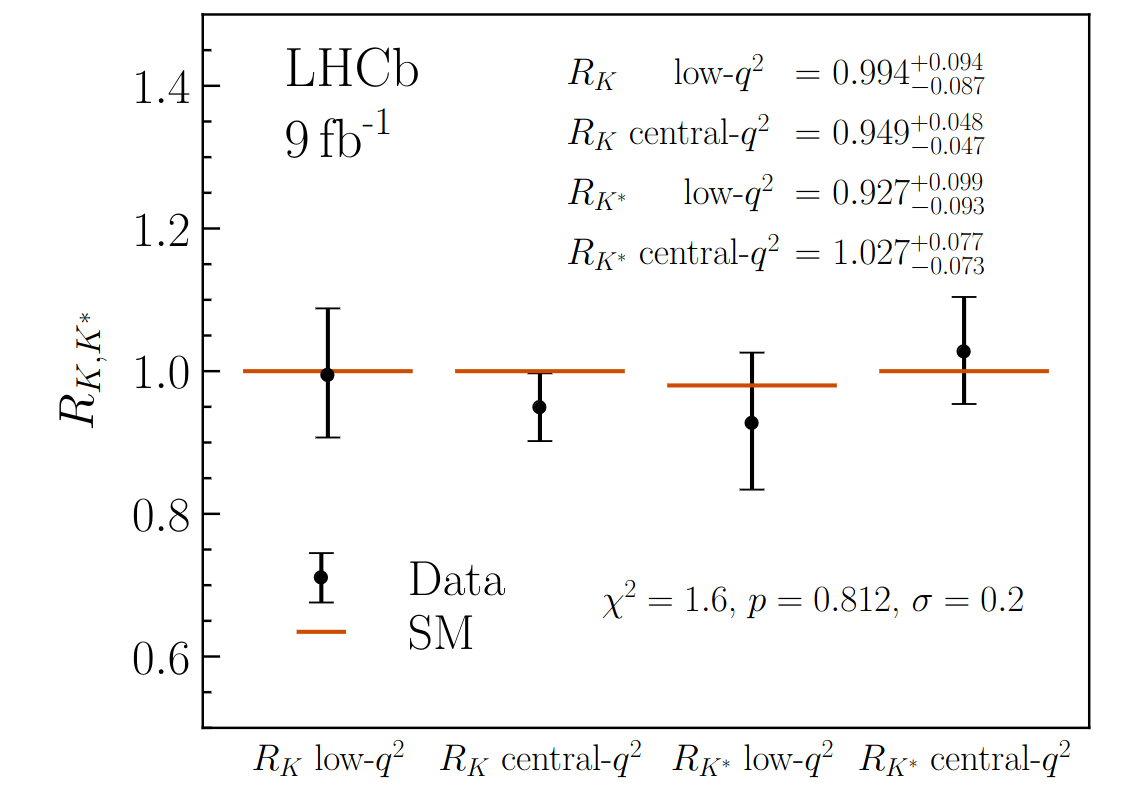
\includegraphics[width=0.5\textwidth]{fit.png}
    \caption{Comparison of the LU measurements with the SM prediction. The results of
    both observables agree with the
    SM prediction in both $q^2$ regions.}
    \label{fig:5}
\end{figure}
\bibliography{lit} 
\end{document}
% 
% ****** End of file apssamp.tex ******